\chapter{Current designs to decrease overflow turbidity}
\label{app:current_designs}

The surface turbidity is a problem in the present and future. Certain partial solutions are existing these days, which are described in this appendix. Both solutions are solvers for the air problem. \newline

\noindent \textbf{Green valve / Environmental valve} \newline
The green valve, or so called environmental valve, is a valve which is placed inside the overflow. The valve can be set to certain angles to choke the flow in the overflow in such a way that a constant fluid level in the hopper in maintained and so reduce the plunging manner of inflow. The valve nowadays is integrated in the automation system of the TSHD and entering a few settings is sufficient to activate the system. Pump velocity, dredged concentration, amount of pumps are some things the automatic system works with. A picture of an environmental valve is shown in figure \ref{fig:Env_valve}.

\begin{figure}[ht!]
    \centering
    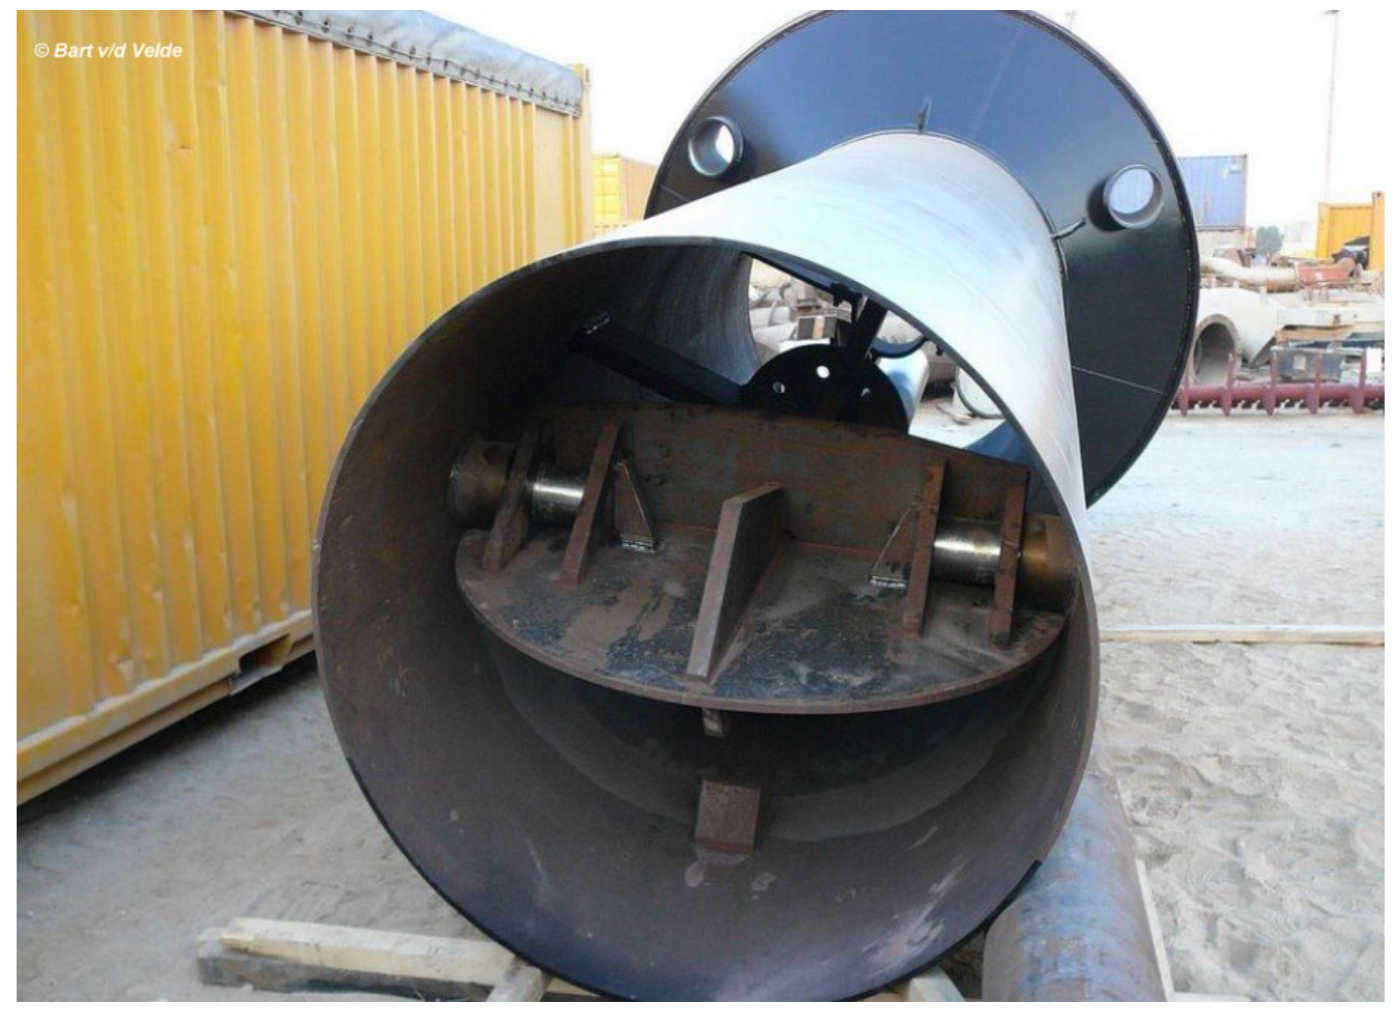
\includegraphics[width =0.6\textwidth]{Images/Green_valve.png}
    \caption{Environmental valve inside the overflow}
    \label{fig:Env_valve}
\end{figure}

\noindent Numerical research is done investigating the environmental valve, for example by \citep{Saremi+} and \citep{Decrop}. \cite{Saremi+} created a two-phase numerical model implemented in OpenFOAM based on the Volume of Fluid method \citep{Hirt+}. This numerical model is used to simulate the performance of the environmental valve. Figure \ref{fig:Env_valve_1} shows the air-water interface from the CFD results.

\begin{figure}[ht!]
    \centering
    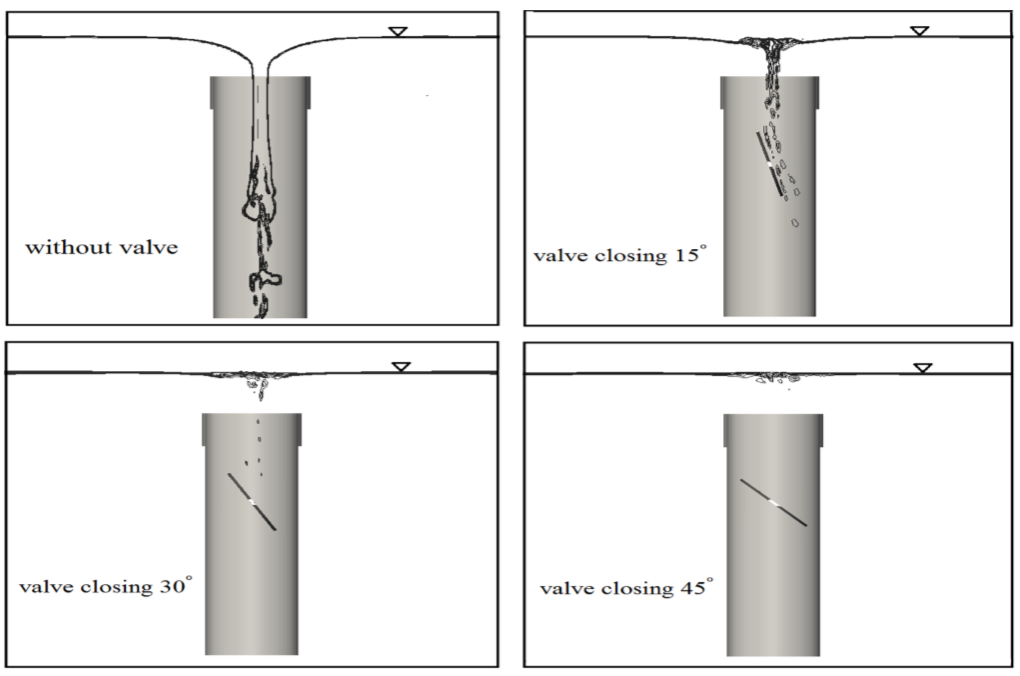
\includegraphics[width =0.6\textwidth]{Images/Env_valve_1.png}
    \caption{Air-water interface from the CFD results}
    \label{fig:Env_valve_1}
\end{figure}

\noindent The numerical results confirm the effectiveness of the valve in reducing the rate of entrainment of the air bubbles into the overflow. The presence of the valve causes an extra hydraulic resistance to the flow passing through the shaft and reduces the flow rate. This reduction results in smaller Froude numbers inside the shaft and therefore reduces the critical submergence at the shaft intake which then results in less air entrainment. \newline
The results from the numerical model also show the reduction in the flow rate through the shaft (figure \ref{fig:Env_valve_2}), which is always been considered as a draw back of using the green valve. However, the results tell that the rate of reduction in the air entrainment due to closure of the valve is far more higher than the relative reduction in the flow rate for the corresponding valve closure.

\begin{figure}[ht!]
    \centering
    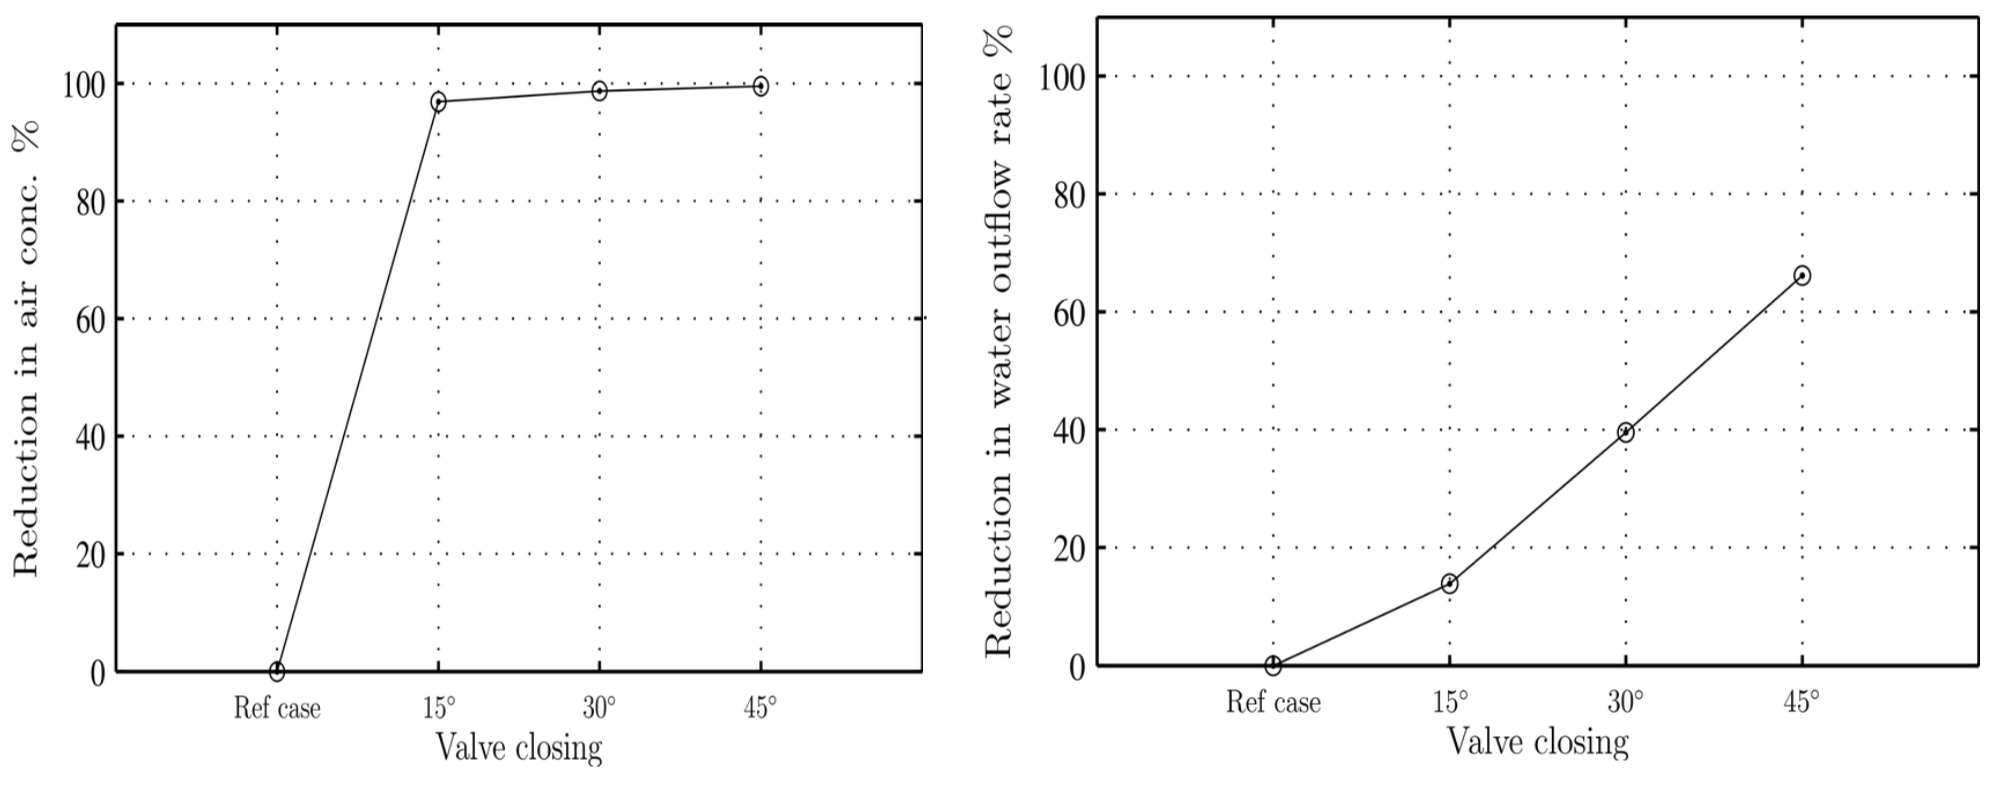
\includegraphics[width =1\textwidth]{Images/Env_valve_2.png}
    \caption{Reduction in air entrainment (left) and water flux (right)}
    \label{fig:Env_valve_2}
\end{figure}

\noindent \cite{Decrop} concluded that the environmental valves indeed can reduce the surface plumes with a high efficiency in many cases. However, it is also shown that under certain circumstances the efficiency can drop significantly, to nearly zero in some cases. It is shown that the valve efficiency is a function of (i) the distance from the overflow to the stern, (ii) the overflow shaft diameter, (iii) the overflow sediment concentration and (iv) the relative speed of the vessel through
the water. \newline
It was found that an environmental valve positioned close to the stern increases the probability that the efficiency will drop during operation. In case of such unfavourable overflow position, the operation of the vessel is dominant in the valve's efficiency. In case an unfavourable overflow position is combined with a high sailing speed or head-on current, the efficiency of the valve drops to nearly zero. \newline
On the other hand, in case of a favourable overflow construction - a narrow shaft, positioned at large distance from stern - only exceptional operational circumstances will reduce the efficiency of the valve significantly. \newline 

\noindent The environmental valve is a great way to decrease the surface plume of a TSHD. However, the main drawback is the valve it self which is located in the overflow and so hard reachable to maintain. Also the valve has moving parts which will suffer from the water-sediment mixture that flows trough the overflow and so must be replaced every now and then. These factors brought to the fact that another solution could be investigated.



\newpage

%%%%%%%%%%%%%%%%%%%%%%%%%%%%%%%%%%%%%%%%%%%%%%%%%%%
\noindent \textbf{Royal IHC Plumigator® Overflow} \newline
In 2017, \cite{IHC} came with the patented plumigator® overflow which is an upgrade to the telescopic overflow system. It is designed to guarantee an optimal, non-turbulent flow inside the hopper. Additional, the plumigator® overflow has no additional moving parts unlike the traditional green valve, is an integration with newly-built vessels or can be retrofitted to current TSHD's and has a reduction of a vessel's ecological impact. An image of the plumigator® overflow is shown below in figure \ref{fig:IHC}.

\begin{figure}[ht!]
    \centering
    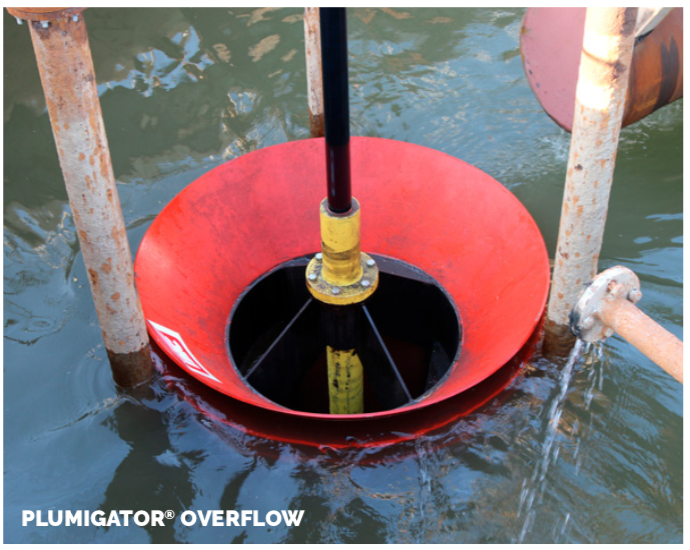
\includegraphics[width =0.6\textwidth]{Images/IHC.png}
    \caption{Royal IHC Plumigator® Overflow}
    \label{fig:IHC}
\end{figure}

\noindent Royal IHC claims that the plumigator® overflow tackles the undesirable plume created around the vessel, which is know to harm marine life. A loss of performance can also be incurred, as well as additional downtime and maintenance costs. In addition, draft sensors can sometimes give inaccurate readings, which can have an impact on overall vessel performance. \newline 
\noindent The issues occur when air is released beneath the vessel by the regular overflow. This combines with entrapped fine soil particles, and the mixture remains near the hull.
As it moves through the propellers, a large surface area will be covered and this appears as a plume. By entering the intake valves of the pumps and auxiliary equipment, the performance and lifetime of the system are affected. \newline
\noindent Royal IHC claims that the patented design significantly limits the influx of air in the overflow, and contributes to a hassle-free operation. The multiple inlet openings also reduce the velocity in the hopper, allowing the mixture extra time to settle. However, the amount of influx of air that is reduced is not made public.